\subsection{Sprint 4: 10.04 \textendash 02.05.2026}\label{subsec:sprint-4}

\subsubsection{Sprint Planning 4: 09.04.2026}\label{subsubsec:sprint-planning-4}

\begin{table}[H]
    \centering
    \begin{tabularx}{\textwidth}{l l X}
		\toprule
        \textbf{Week} & \textbf{Responsible} & \textbf{Task} \\
        \midrule
        Week 1 & Frank \& Lukas & Bring together and test reproducible test environment and \gls{AI} Reconnaissance \\
        Week 2 \& 3 & Frank & Network Discovery - Red Team  \\
        Week 2 & Lukas & \gls{NSAK} Scenario: \gls{AI} Scenarios (second part): Improve tool calling and documentation \\
        Week 3 & Lukas & External Logging with Grafana / Loki \\
        \bottomrule
    \end{tabularx}
    \caption{Sprint Planning 3}
    \label{tab:sprint-planning-4}
\end{table}

\subsubsection{Sprint Review 4: 02.05.2026}\label{subsubsec:sprint-review-4}

In this sprint could finally bring together the reproducible network environment and the \gls{AI} scenario,
we realized the last scenario categorized as \enquote{Must} goal,
extended the logging capabilities and could refine the \gls{AI} agent.
Now we can focus on refining the documentation and finalizing the last preparations before moving to the last phase of our thesis, the evaluation and discussion.

\paragraph{Test run of the \gls{AI} scenario in the reproducible network environment}\label{par:test-run-of-ai-scenario-in-the-reproducible-network-environment}

After finishing the previous sprint we were excited to test the \gls{AI} scenario in the reproducible network environment,
as it's marking a big milestone of our bachelor thesis.
We spent more or less a whole day using different models and make fine adjustments to the setup, to see what's possible.
In the end we could instruct the \gls{AI} agent to conduct network discovery, write a report in markdown, create a network diagram of the findings
and send the artifacts via E-Mail.
The results of this test run where added to the implementation section of the thesis~\ref{subsubsec:scenario-ai-reconnaissance-test-run}.

\paragraph{Milestone Review: Network Discovery - Red Team}\label{par:milestone-review-network-discovery-red-team}

In~\ref{fig:milestone-network-discovery-red-team}, not all \enquote{must} goals of the milestone where completed.
During planning, a human interaction mode was discussed in which an operator could choose how fast or noisy the reconnaissance should be executed.
This feature was not implemented, as it does not contribute to answering the thesis question.
The scenario is able to discover MAC and IP addresses using arp-scan on Layer~2, and protocols and services using nmap within the local subnet.
All results are stored in a \texttt{NetworkDiscoveryResultMap} and displayed to the operator.
Service enumeration using targeted \gls{NSE} scripts was implemented as a dedicated drill, which runs service-specific scripts such as \texttt{http-title}, \texttt{dns-zone-transfer}, and \texttt{smb-security-mode} on all discovered ports.

The scenario could be extended with an optional static IP address, which would be useful in networks where \gls{DHCP} is not available.
Host discovery in remote networks is currently limited to IP addresses only, as \gls{MAC} addresses are not available across Layer~3 boundaries.

\todo{Maybe move the content to the implementation section and reference it}

\begin{figure}[H]
    \centering
    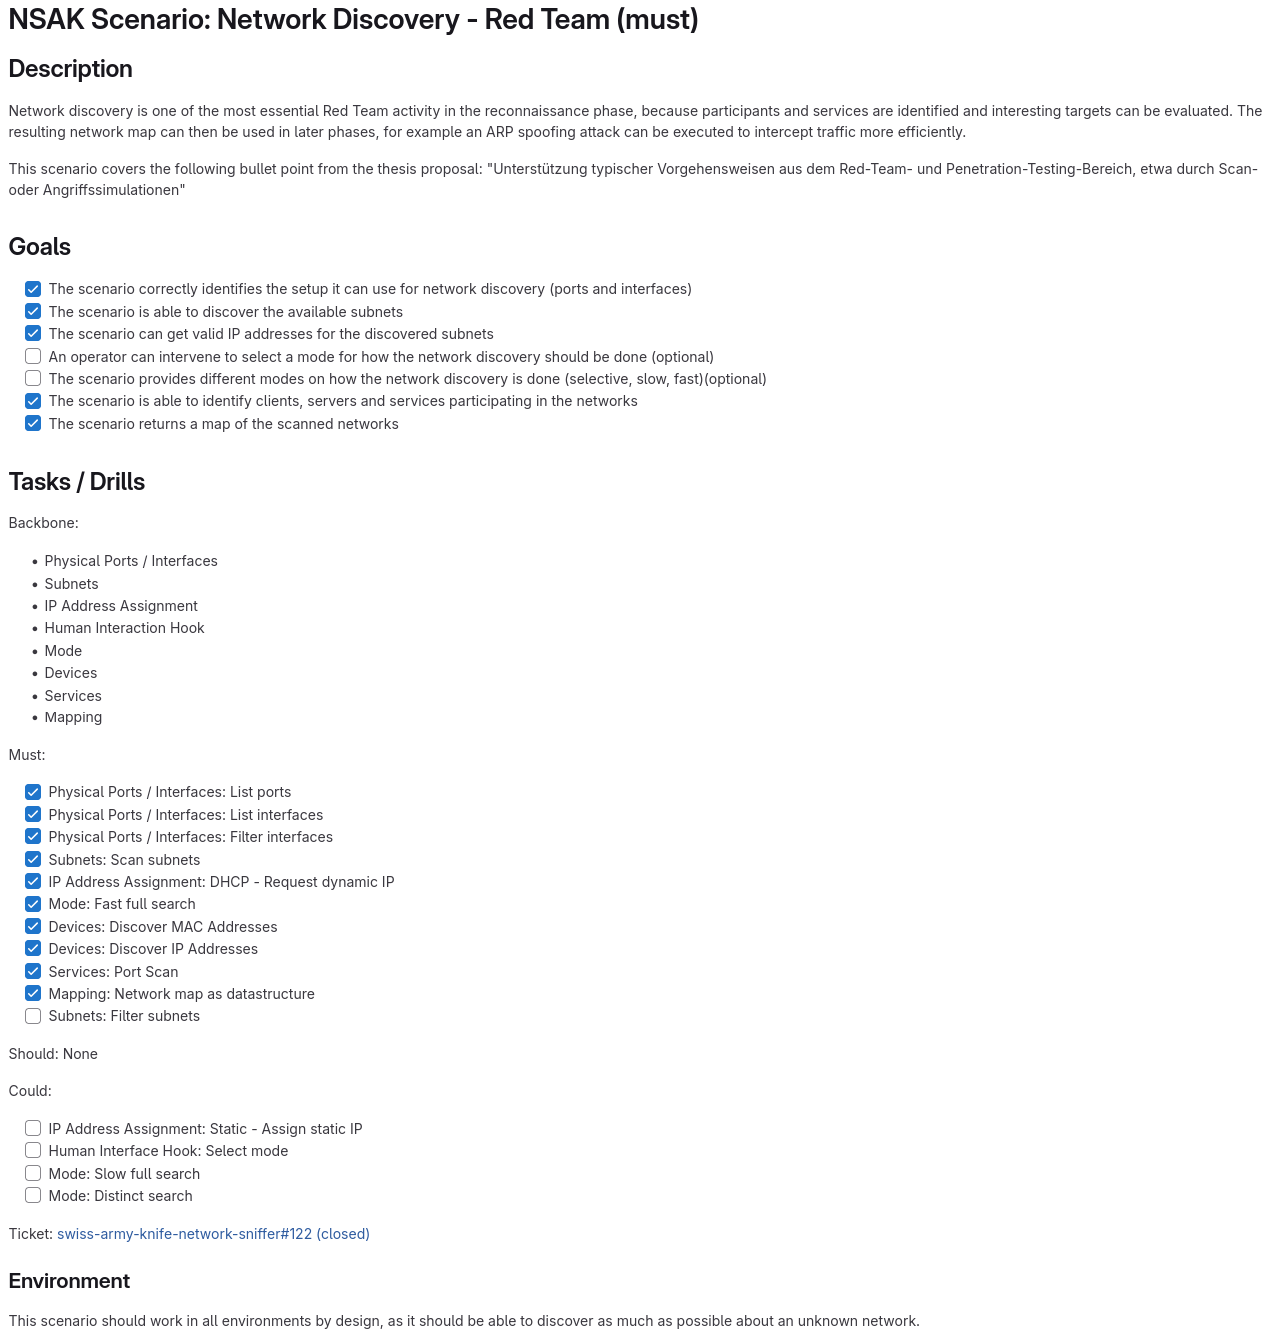
\includegraphics[width=1.0\linewidth]{../assets/screenshots/project_management/sprint_4/network_discovery_red_team}
    \caption{Milestone Description: Reproducible Test Environment}
    \label{fig:milestone-network-discovery-red-team}
\end{figure}

\paragraph{Milestone Review: Implement AI Scenarios (second part): Improve tool calling and documentation}\label{par:milestone-review-implement-ai-scenarios-second-part}

As already shown in~\ref{fig:milestone-review-implement-ai-scenarios]} from the previous sprint review~\ref{subsubsec:sprint-review-3}, all \enquote{must} goals of the milestone Implement \gls{AI} Scenarios~\ref{subsubsec:milestone-ai-scenarios} where completed.
In this second part the \gls{AI} scenarios where tested, tool calling was improved and the documentation was added to the implementation section of the thesis~\ref{sec:ai-scenarios-implementation}.
Further we could already improve the \gls{AI} scenarios with the findings of the extensive test run described above~\ref{par:test-run-of-ai-scenario-in-the-reproducible-network-environment}.

\paragraph{External Logging with Grafana / Loki}

In the fifth checkpoint meeting~\ref{subsec:checkpoint-meeting-5} which as in this sprint,
we received the feedback that we should improve the logging for the \gls{AI}-agent and especially which tools it is calling.
We decided to set up a self-hosted logging system with Grafana and Loki, where we can collect all logs of the runs and
create custom queries to make it easier to analyze the behavior of the \gls{AI}-agent.
The usage is described in the implementation section of the \gls{AI} Scenarios~\ref{subsubsec:ai-scenarios-implementation-remote-logging-system}.
The self-hosted setup is documented in the addendum~\ref{subsec:grafana-loki-logging-system}.

\subsubsection{Sprint Retro 4: 02.05.2026}\label{subsubsec:sprint-retro-4}

\textbf{Key Takeaways:}

\begin{itemize}
    \item Overall good mood and good progress
    \item Use 80/20 rule for documentation during the implementation phase, so that the base structure is already there.
    \item Work more continuously on the Bachelor Thesis during the Week (1-2h every day)
\end{itemize}

\begin{figure}
    \centering
    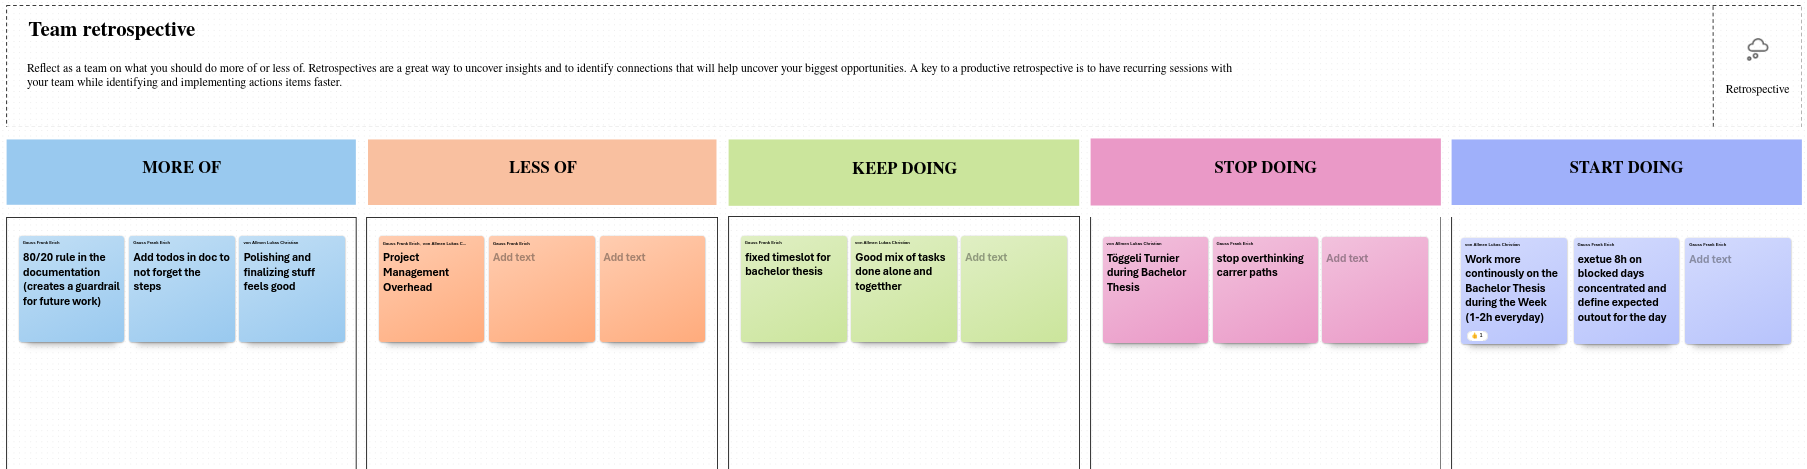
\includegraphics[width=0.7\linewidth]{../assets/screenshots/project_management/sprint_4/retro_sprint_4}
    \caption{Retro Sprint 4}
    \label{fig:retro-sprint-4}
\end{figure}
